\documentclass{article}

\usepackage{defines}

\begin{document}

\tickettitle{8}{Теорема о геометрическом смысле декартовых координат в трехмерном пространстве. Деление вектора в заданном соотношении.}

\define{геометрической проекции (меры) в $\A^{3}$}

\begin{minipage}{0.6\linewidth}
	\begin{enumerate}
		\item{}$O\vec{e}_{1}\vec{e}_{2}\vec{e}_{3}$ --- аффинная система координат
		\item{}$A:\lvec{OA}=\vec{a}$
		\item{}$A':=A\vec{e}_{1}\vec{e}_{2}\cap O\vec{e}_{3}$
	\end{enumerate}
	\begin{align*}
		 & \Proj_{\vec{e}_{3}}\vec{a}:=\lvec{OA'} &  & \Apr_{\vec{e}_{3}}\vec{a}=OA'
	\end{align*}
	Аналогично определяются $\Proj_{\vec{e}_{1}}$ и $\Proj_{\vec{e}_{2}}$
\end{minipage}%
\begin{minipage}{0.4\linewidth}
	\centering
	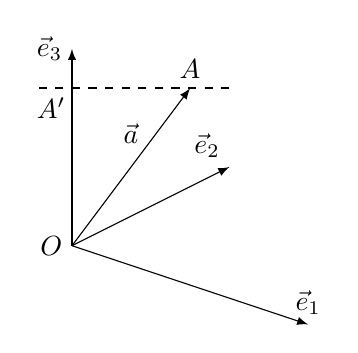
\begin{tikzpicture}
		\filldraw (0,0) node[anchor=east] {$O$};
		\filldraw (1.5,2) node[anchor=south] {$A$};
		\filldraw (0,2) node[anchor=north, xshift=-0.75em] {$A'$};
		\draw [-latex] (0,0)--(2,1) node[above left] {$\vec{e}_{2}$};
		\draw [-latex] (0,0)--(3,-1) node[above] {$\vec{e}_{1}$};
		\draw [-latex] (0,0)--(0,2.5) node[left=] {$\vec{e}_{3}$};
		\draw [-latex] (0,0)--(1.5,2) node[midway, above=0.5em] {$\vec{a}$};
		\draw [dashed, thick] (2,2)--(-0.5,2);
	\end{tikzpicture}
	\captionof{figure}{Proj в $\A^{3}$}
\end{minipage}

\theorem

Координаты $\vec{a}$ в аффинной системе координат $O\vec{e}_{1}\vec{e}_{2}\vec{e}_{3}$ --- $\left(\Apr_{\vec{e}_{1}}\vec{a},\Apr_{\vec{e}_{2}}\vec{a},\Apr_{\vec{e}_{3}}\vec{a}\right)$

\proof

Используя обозначения из определения:
\begin{align*}
	 & \vec{a}=\lvec{OA}=\lvec{OA'}+\lvec{A'A}=\left(\Apr_{\vec{e}_{3}}\vec{a}\right)\vec{e}_{3}+\lvec{A'A}                                                                       \\
	 & \lvec{A'A}\subset O\vec{e}_{1}\vec{e}_{2}\Rarr \lvec{A'A}=\lambda_1\vec{e}_{1}+\lambda_2\vec{e}_{2}                                                                        \\
	 & \vec{a}=\left(\Apr_{\vec{e}_{3}}\vec{a}\right)\vec{e}_{3}+\lambda_1\vec{e}_{1}+\lambda_2\vec{e}_{2}\Rarr \Apr_{\vec{e}_{3}}\vec{a}\text{ --- третья координата $\vec{a}$ }
\end{align*}

Аналогично $\Apr_{\vec{e}_{1}}\vec{a}$ --- первая координата, $\Apr_{\vec{e}_{2}}\vec{a}$ --- вторая координата.

Таким образом, $\left(\Apr_{\vec{e}_{1}}\vec{a},\Apr_{\vec{e}_{2}}\vec{a},\Apr_{\vec{e}_{3}}\vec{a}\right)$ --- координаты $\vec{a}\qed$

\define{деления вектора в заданном соотношении}

Точка $M\neq B$ делит вектор $\lvec{AB}$ в соотношении $\lambda\neq -1$, если $\lvec{AM}=\lambda\lvec{MB}$, $M\in AB$
\begin{align*}
	\vec{r}_{M}-\vec{r}_{A}=\lambda\left(\vec{r}_{B}-\vec{r}_{M}\right)\Rarr \vec{r}_{M}=\frac{\vec{r}_{A}+\lambda\vec{r}_{B}}{1+\lambda}
\end{align*}

Определеим координатный вектор $\vec{e}_{1}\parallel\lvec{AB}$ и выразим $\lambda$ с помощью $\mes_{\vec{e}_{1}}$:
\begin{align*}
	\mes_{\vec{e}_{1}}\lvec{AM}=\mes_{\vec{e}_{1}}\left(\lambda\lvec{MB}\right)\Rarr
	\mes_{\vec{e}_{1}}\lvec{AM}=\lambda\mes_{\vec{e}_{1}}\lvec{MB}\Rarr
	\lambda=\frac{\mes_{\vec{e}_{1}}\lvec{AM}}{\mes_{\vec{e}_{1}}\lvec{MB}}
\end{align*}

\end{document}
